\documentclass[12pt]{amsart}
\usepackage{amsmath, amssymb, amsthm}
\usepackage[margin=2.5cm]{geometry}
\usepackage{xr-hyper}
\usepackage{hyperref}
\usepackage{xurl}
\usepackage{booktabs}
\usepackage{graphicx}
\emergencystretch=2em

\newtheorem{theorem}{Theorem}
\newtheorem{corollary}[theorem]{Corollary}
\newtheorem{proposition}[theorem]{Proposition}
\newtheorem{conjecture}[theorem]{Conjecture}
\newtheorem{lemma}{Lemma}
\renewcommand{\thelemma}{\Alph{lemma}}
\theoremstyle{remark}
\newtheorem{remark}{Remark}

\newcommand{\E}{\mathbb{E}}
\newcommand{\Et}{\widetilde{\mathbb{E}}}
\newcommand{\eps}{\varepsilon}
\newcommand{\T}{\mathbb{T}}
\newcommand{\1}{\mathbf{1}}
\newcommand{\sinc}{\operatorname{sinc}}
\DeclareMathOperator{\Var}{Var}
\externaldocument[S-]{arxiv_small_gap_hump_supp}

\title[The hump between two close zeros]{The hump between two close
zeros:\\ random unitary matrices and the Riemann zeta function}

\author{U\u{g}ur Sezen}
\address{Independent researcher, Istanbul, Turkey}
\email{usezen@aof.anadolu.edu.tr}

\date{\today}

\begin{document}

\begin{abstract}
Let $M$ be the maximum of $|\Lambda_N|$, the characteristic polynomial of
a Haar unitary $N\times N$ matrix, on the arc between two consecutive
eigenangles at distance $s$. For fixed $N$ we prove that, conditionally on
$s<\eps$, the pair $(s/\eps, M/s^2)$ converges in law as $\eps\to0$ to
independent variables $(U^{1/3}, X_{N-2}/4)$, where $U$ is uniform and
$X_{N-2}$ is $|\Lambda_{N-2}(1)|$ under the $|\Lambda_{N-2}(1)|^4$-tilted
Haar measure. Such gaps occur at rate $N^2(N^2-1)\eps^3/(72\pi)$, and by
the product formula of Bourgade, Hughes, Nikeghbali and Yor all moments and
log-cumulants of the hump are explicit; in unfolded units the log-hump has
mean $\to2\log\pi+2\gamma-10/3$ and a negative third cumulant
$\to-0.1271$. For the Riemann zeros we cast the analogue as a tilt ladder,
conditioning on $b=0,1,2$ zeros, and test it on zeros at heights
$L=\log(t/2\pi)\approx9$--$22$. On the first two rungs,
$\log|\zeta(\frac12+it)|$ and $\log|\zeta'(\rho)|$, we derive the variance
and the third cumulant at finite height from the ratios conjecture, using
three- and four-point averages of $\zeta'/\zeta$ and the density of zeros;
the identity term reproduces the constant of Fazzari and Gerspach. Without
free parameters the four predictions match the data at all seven heights
($\chi^2$ between $2.5$ and $11.6$ for $7$ points), while the random-matrix
model with the Keating--Snaith arithmetic factor, which is right in the
limit, fails at these heights ($\chi^2$ up to $16\,826$). Pre-registered
tests also show that midpoints of close pairs lock to the phases of the
prime waves about four times as strongly as single zeros.
\end{abstract}

\maketitle

%======================================================================
\section{Introduction}
%======================================================================

Let $\gamma_n<\gamma_{n+1}$ be consecutive ordinates of zeros of the
Riemann zeta function on the critical line, $\delta_n=\gamma_{n+1}-\gamma_n$,
and let $M_n=\max_{\gamma_n\le t\le\gamma_{n+1}}|Z(t)|$ be the height of
Hardy's function between them. The mean of $M_n^2$ over all gaps is known
\cite{CG85,HLPC24}; the \emph{joint} law of $(\delta_n,M_n)$ was studied
numerically in \cite{companion1}, whose first open problem asked for the
mean of $M_n^2$ conditioned on the gap. A reader asked the sharper
question: in the regime of asymptotically small gaps, can the joint
distribution of $(\delta_n,M_n^2)$ be determined?

For random unitary matrices the answer is yes, and exact. When two zeros
nearly coincide, the hump between them is crushed by the square of the
gap, and what is left is the height produced at the collision point by all
the \emph{other} zeros. For the characteristic polynomial of a Haar
unitary matrix, conditioning two eigenvalues to merge at a point tilts the
remaining $N-2$ eigenvalues by $|\Lambda_{N-2}|^4$ at that point; under
this tilt the value $|\Lambda_{N-2}|$ is a product of independent factors,
so every moment and every cumulant of the logarithm is explicit.

\subsection*{Results for the unitary group}
Let $s$ be a gap between consecutive eigenangles of $U\in U(N)$ and $M$ the
maximum of $|\Lambda_N|$ on it (Section~\ref{sec:setup}).
\begin{itemize}
\item \emph{Theorem~\ref{thm:main}} (fixed $N$, $\eps\to0$). The expected
number of gaps below $\eps$ is $N^2(N^2-1)\eps^3/(72\pi)\,(1+o(1))$;
conditionally on $s<\eps$ (for a gap chosen uniformly),
$(s/\eps, M/s^2) \Rightarrow (U^{1/3}, X_{N-2}/4)$ with $U$ uniform on
$[0,1]$ and \emph{independent} of $X_{N-2}$, the value $|\Lambda_{N-2}(1)|$
under the $|\Lambda_{N-2}(1)|^4$-tilted Haar measure. All moments
$\E(M/s^2)^{2k}$ with $k>-5/2$ and all log-moments converge; the threshold
is sharp.
\item \emph{Theorem~\ref{thm:product}}. $X_n$ has the law of
$\prod_{j=1}^n|1-\xi_j|$ with independent, explicitly distributed $\xi_j$;
$\E X_n^{2k}$ is a ratio of Keating--Snaith moments and
$\kappa_r(\log X_n)=\sum_{j=1}^n[\psi^{(r-1)}(j+4)-2^{1-r}\psi^{(r-1)}(j+2)]$.
\item \emph{Corollary~\ref{cor:largeN}} (large $N$, unfolded units). The
moments grow like $N^{k^2}$ with the constant
$\pi^{4k}\,12\,G(k+3)^2/G(2k+5)$; the log-hump has mean
$\to2\log\pi+2\gamma-10/3$, variance $\tfrac12\log N+c_2+o(1)$ with
$c_2=65/18+\gamma/2-\pi^2/2$, third cumulant negative for every $N$ and
tending to $-0.127077$, and is asymptotically Gaussian.
\item Small gaps are invisible in the second moment: gaps below
$\tilde\eps$ in unfolded units carry a share of order $\tilde\eps^{\,7}$ of
$\E\sum_nM_n^2\sim\frac{e^2-5}2N^2$, the constant being Winn's
\cite{Win12} (Section~\ref{S-sec:second} of the Supplementary material).
\end{itemize}

\subsection*{What is known}
To our knowledge, the joint (gap, hump) law has not been written down
before, but its ingredients are known. That conditioning the eigenvalues
on points at a given location tilts the remaining points by powers of the
characteristic polynomial is the Palm-measure structure of these ensembles
(for the unitary group it is immediate from Weyl's formula; see
\cite{For10} for the log-gas setting). The Haar measure tilted by
$|\det(1-U)|^{2\delta}$ is the circular Jacobi ensemble \cite{For10,BNR09},
which for $\delta\in\mathbb N$ is the CUE conditioned to have $\delta$
further eigenvalues at $1$ \cite[\S1.1]{BNR09}, and the product formula for
$\det(1-U)$ under Haar and tilted measures is due to Bourgade, Hughes,
Nikeghbali and Yor \cite{BHNY08} and Bourgade, Nikeghbali and Rouault
\cite{BNR09}. Theorem~\ref{thm:product} is a direct consequence of their
results and is presented as such. The small gaps of the CUE were
determined by Ben Arous and Bourgade \cite{BAB13} (Poisson limit at scale
$N^{-4/3}$; Theorem~\ref{thm:main}(a) agrees with their intensity), and
small gaps of other ensembles in \cite{FTW19,FW21,Bou22}; these works
concern the gaps, not the polynomial between the eigenvalues. Joint
moments of the characteristic polynomial and its derivatives in the
circular Jacobi ensemble have recently been related to Painlev\'e
equations \cite{BW26}; conditioning on coalescing eigenvalues is not
considered there. The proof of Theorem~\ref{thm:main} is elementary
(Weyl's formula and dominated convergence); the negative moments require a
uniform domination, which follows from a one-line geometric inequality
(Lemma~\ref{lem:dom}).

\subsection*{The zeta side}
Conditioning on $b$ zeros at a point tilts the rest of the spectrum by
$|\Lambda|^{2b}$: $b=0$ is the value distribution of $\log|\zeta|$
(Keating--Snaith \cite{KS00}), $b=1$ is $\log|\zeta'(\rho)|$
(Hughes--Keating--O'Connell \cite{HKO00}; see \cite{BGM15}), and $b=2$ is
the log-hump of close pairs studied here. Adding the Keating--Snaith
arithmetic factor $a_k$ to each rung gives a parameter-free prediction for
the cumulants (Section~\ref{sec:zeta}), which we tested in pre-registered
steps on Riemann zeros (Section~\ref{sec:tests}). The arithmetic shift of
the variance is nearly rung-independent and close to that of $a_k$, but the
arithmetic shift of the third cumulant decreases from
rung to rung at $L\approx9$--$12$ --- a decrease that was predicted blind
for $b=2$ from the two lower rungs --- and the ladder flattens as the height
grows. On the first two rungs this finite-height behaviour is now
accounted for without free parameters (Section~\ref{sec:ratios}): the
ratios conjecture of Conrey, Farmer and Zirnbauer, evaluated with three-
and four-point averages of $\zeta'/\zeta$ that we derive
(Appendix~\ref{app:ratios}) and weighted by the density of zeros, gives
the variance and the third cumulant of $\log|\zeta(\frac12+it)|$ and of
$\log|\zeta'(\rho)|$ at each height, and all four match the data
(Figure~\ref{fig:ladder}). The close-pair rung $b=2$ remains open. A
further pre-registered test finds that midpoints of close pairs lock to the
phases of the prime waves about four times as strongly as single zeros, as
a local-GUE heuristic predicts; this lock has the predicted size and does
not by itself explain the decay along the ladder. We report the failed parts of the predictions next to the
successful ones. Nothing here bears on a proof of the Riemann Hypothesis.

Complements to the proofs, the second-moment computation, the full Monte
Carlo record and the complete protocol and results of the pre-registered
tests are in the Supplementary material, whose sections are numbered
S1--S8.

%======================================================================
\section{Setup and notation}\label{sec:setup}
%======================================================================

\subsection*{Eigenangles}
Let $U$ be Haar distributed on $U(N)$, $N\ge2$, with eigenvalues
$e^{i\theta_1},\dots,e^{i\theta_N}$, the labelled eigenangles
$\theta=(\theta_1,\dots,\theta_N)\in\T^N$, $\T=[0,2\pi)$, being
exchangeable with density (Weyl's integration formula)
\begin{equation}\label{eq:weyl}
p_N(\theta)=\frac{1}{(2\pi)^N N!}\prod_{1\le j<k\le N}
|e^{i\theta_j}-e^{i\theta_k}|^2 .
\end{equation}
The density is invariant under the rotation
$\theta_j\mapsto\theta_j+\alpha$; almost surely the $\theta_j$ are
distinct. For $n\ge0$ we write $\E_n$ for the expectation under
$p_n$ ($\E_0$ is trivial) and
\[
|\Lambda_n(e^{i\vartheta})| = \prod_{j=1}^n|e^{i\vartheta}-e^{i\theta_j}|
=\prod_{j=1}^n 2\Big|\sin\frac{\vartheta-\theta_j}{2}\Big|,
\qquad \Lambda_0\equiv1,
\]
for the modulus of the characteristic polynomial $\det(e^{i\vartheta}-U)$;
only the modulus is used.

\subsection*{Keating--Snaith moments}
For $n\ge1$ and real $k$,
\begin{equation}\label{eq:KS}
\mathcal M_n(k):=\E_n|\Lambda_n(1)|^{2k}
=\prod_{j=1}^n\frac{\Gamma(j)\Gamma(j+2k)}{\Gamma(j+k)^2}
\qquad (k>-\tfrac12),
\end{equation}
and $\mathcal M_n(k)=\infty$ for $k\le-\frac12$ \cite{KS00} (see also the
proof of Theorem~\ref{thm:main}(c)); $\mathcal M_0\equiv1$. By rotation
invariance $\E_n|\Lambda_n(e^{i\alpha})|^{2k}=\mathcal M_n(k)$ for every
$\alpha$. Telescoping the products gives
\begin{equation}\label{eq:M23}
\begin{aligned}
\mathcal M_n(2)&=\frac{(n+1)(n+2)^2(n+3)}{12},\\
\mathcal M_n(3)&=\frac{(n+1)(n+2)^2(n+3)^3(n+4)^2(n+5)}{8640}.
\end{aligned}
\end{equation}

\subsection*{Gaps and humps}
Order the eigenangles, $\theta_{(1)}<\dots<\theta_{(N)}$, put
$\theta_{(N+1)}=\theta_{(1)}+2\pi$, and let
\[
s_n=\theta_{(n+1)}-\theta_{(n)},\qquad
M_n=\max_{\theta_{(n)}\le\vartheta\le\theta_{(n+1)}}|\Lambda_N(e^{i\vartheta})|,
\qquad n=1,\dots,N .
\]
The unfolded gap is $\tilde s_n=Ns_n/2\pi$ (mean one). For a function
$G_n$ of the $n$-th gap we write
\begin{equation}\label{eq:palm}
\langle G\rangle_\eps:=\frac{\E\sum_{n=1}^N\1\{s_n<\eps\}G_n}
{\E\#\{n:s_n<\eps\}}=\E\big[G_J\,\big|\,s_J<\eps\big],
\end{equation}
where $J$ is uniform on $\{1,\dots,N\}$ and independent of $U$: this is the
law of a typical gap conditioned to be small.

\subsection*{The tilted law}
For $n\ge1$ let $\widetilde{\mathbb P}_n$ be the Haar measure of $U(n)$
tilted by $|\Lambda_n(1)|^4/\mathcal M_n(2)$, $\Et$ its
expectation, and $X_n$ the random variable $|\Lambda_n(1)|$ under
$\widetilde{\mathbb P}_n$. This is the circular Jacobi ensemble of
\cite[Def.~1.1]{BNR09} with $\beta=2$ and $\delta=2$: their weight
$(1-e^{-i\theta_j})^{\delta}(1-e^{i\theta_j})^{\bar\delta}$ equals
$|1-e^{i\theta_j}|^{2\delta}$ for real $\delta$. Thus
\[
\Et\, h(X_n)=\frac{\E_n\big[|\Lambda_n(1)|^4\,h(|\Lambda_n(1)|)\big]}
{\mathcal M_n(2)} .
\]
We set $X_0\equiv1$. In unfolded units the limit object is
$Y_N:=(2\pi/N)^2X_{N-2}/4$.

\subsection*{Special functions}
$H_m^{(r)}=\sum_{i=1}^m i^{-r}$, $H_m=H_m^{(1)}$; $\psi=\Gamma'/\Gamma$
and $\psi^{(r)}$ its derivatives; $\gamma$ is Euler's constant; $G$ is the
Barnes function, $G(z+1)=\Gamma(z)G(z)$, $G(1)=1$;
$\sinc x=\sin x/x$. Cumulants are $\kappa_r$.

%======================================================================
\section{The small-gap limit}\label{sec:thm1}
%======================================================================

\begin{theorem}\label{thm:main}
Let $N\ge2$ and $B_N:=2^{N-2}/4$.
\begin{enumerate}
\item[(i)] For every configuration of distinct eigenangles and every $n$,
$0<M_n/s_n^2\le B_N$.
\item[(ii)] Let $F:(0,1]\times(0,B_N]\to\mathbb R$ be continuous, and
suppose that $|F(u,y)|\le C(1+y^{2k_0})$ for some $C<\infty$ and some
$k_0\in(-\frac52,0]$. Then
\begin{equation}\label{eq:main}
\lim_{\eps\downarrow0}\;\eps^{-3}\,
\E\sum_{n=1}^N\1\{s_n<\eps\}\,F\Big(\frac{s_n}{\eps},\frac{M_n}{s_n^2}\Big)
=\frac1{2\pi}\int_0^1u^2\,
\E_{N-2}\Big[|\Lambda_{N-2}(1)|^4\,
F\Big(u,\frac{|\Lambda_{N-2}(1)|}{4}\Big)\Big]\,du .
\end{equation}
\end{enumerate}
In particular:
\begin{enumerate}
\item[(a)] $\E\#\{n:s_n<\eps\}=\dfrac{N^2(N^2-1)}{72\pi}\,\eps^3\,(1+o(1))$.
\item[(b)] Under $\langle\cdot\rangle_\eps$,
$(s_J/\eps,\,M_J/s_J^2)\Rightarrow(U^{1/3},\,X_{N-2}/4)$ as $\eps\to0$,
where $U$ is uniform on $[0,1]$ and independent of $X_{N-2}$. In the
small-gap limit, gap and normalised hump are independent.
\item[(c)] For every $k>-\frac52$,
$\langle(M/s^2)^{2k}\rangle_\eps\to4^{-2k}\,\Et X_{N-2}^{2k}
=4^{-2k}\mathcal M_{N-2}(k+2)/\mathcal M_{N-2}(2)$, and for every $m>0$,
$\langle|\log(M/s^2)|^m\rangle_\eps\to\Et|\log(X_{N-2}/4)|^m$; the same
holds for integer powers of $\log(M/s^2)$, so all cumulants of
$\log(M/s^2)$ converge. If $N\ge3$ and $k\le-\frac52$, then
$\langle(M/s^2)^{2k}\rangle_\eps\to\infty$.
\end{enumerate}
\end{theorem}

The factor $|\Lambda_{N-2}(1)|^4$ in \eqref{eq:main} is the product of the
two factors $|\Lambda_{N-2}(e^{i\theta})|^2$ that the Vandermonde
determinant attaches to each of the two merging eigenvalues; $u^2$ is their
mutual repulsion. Ben Arous and Bourgade \cite[Thm.~1.1]{BAB13} showed
that the points $(N^{4/3}(\theta_{(n+1)}-\theta_{(n)}),\theta_{(n)})$
(gaps in angle units) converge to a Poisson process with intensity
$\frac1{24\pi}u^2\,du\,\frac{d\theta}{2\pi}$, so that the mean number of
gaps below $xN^{-4/3}$ tends to $x^3/(72\pi)$; setting $\eps=xN^{-4/3}$ in
(a) gives the same leading term. The two limits are taken in different
orders ($\eps\to0$ at fixed $N$ here, $N\to\infty$ at fixed $x$ there);
the constants agree.

\subsection{Two deterministic lemmas}
Fix $s\in(0,2\pi)$ and a configuration
$\vartheta=(\vartheta_1,\dots,\vartheta_{N-2})\in\T^{N-2}$ of the
remaining angles, with $|\Lambda_{N-2}|$ built from $\vartheta$. Put
\begin{align*}
M(s;\vartheta)&:=\max_{0\le t\le s}\,|e^{it}-1|\,|e^{it}-e^{is}|\,
|\Lambda_{N-2}(e^{it})|,\\
W_s(\vartheta)&:=\prod_{j=1}^{N-2}|e^{i\vartheta_j}-1|^2\,
|e^{i\vartheta_j}-e^{is}|^2,\\
A_s&:=\{\vartheta:\ \vartheta_j\notin(0,s)\ \text{for all } j\}.
\end{align*}
$M(s;\vartheta)$ is the hump over the arc $[0,s]$ of the polynomial with
zeros at $1$, $e^{is}$ and $e^{i\vartheta_j}$; $W_s$ is the Vandermonde
coupling between the pair and the rest; $A_s$ says that the arc is a gap.
For $N=2$ all products over $j$ are empty.

\begin{lemma}[Hump bounds]\label{lem:hump}
For every $s\in(0,2\pi)$ and every $\vartheta$,
\begin{equation}\label{eq:hump}
\frac{4\sin^2(s/4)}{s^2}\,|\Lambda_{N-2}(e^{is/2})|
\;\le\;\frac{M(s;\vartheta)}{s^2}\;\le\;
\frac14\max_{0\le t\le s}|\Lambda_{N-2}(e^{it})|\;\le\;B_N .
\end{equation}
Consequently $M(s;\vartheta)/s^2\to|\Lambda_{N-2}(1)|/4$ as $s\downarrow0$,
for every $\vartheta$; and $M(s;\vartheta)/s^2\ge\frac15|\Lambda_{N-2}(e^{is/2})|$
for $0<s\le1$.
\end{lemma}

\begin{proof}
For $t\in[0,s]$ the numbers $t/2$ and $(s-t)/2$ lie in $[0,\pi)$, so
$|e^{it}-1|=2\sin(t/2)$ and $|e^{it}-e^{is}|=2\sin((s-t)/2)$, and
\[
q_s(t):=4\sin\frac t2\,\sin\frac{s-t}2
=2\Big[\cos\Big(t-\frac s2\Big)-\cos\frac s2\Big].
\]
Thus $q_s$ is maximal at $t=s/2$, where it equals
$2(1-\cos\frac s2)=4\sin^2\frac s4$; evaluating the product at $t=s/2$ gives
the lower bound. Since $0\le\sin x\le x$ for $x\in[0,\pi]$,
$q_s(t)\le t(s-t)\le s^2/4$, which gives the middle bound, and
$|e^{it}-e^{i\vartheta_j}|\le2$ gives the last one. As $s\downarrow0$,
$4\sin^2(s/4)/s^2=\frac14\sinc^2(s/4)\to\frac14$ and both
$|\Lambda_{N-2}(e^{is/2})|$ and $\max_{[0,s]}|\Lambda_{N-2}|$ tend to
$|\Lambda_{N-2}(1)|$ by continuity. Finally, $\sinc$ is decreasing on
$(0,\pi)$, so for $s\le1$, $4\sin^2(s/4)/s^2\ge4\sin^2(1/4)=0.2448\ldots>\frac15$.
\end{proof}

Part (i) of Theorem~\ref{thm:main} follows: after a rotation, the $n$-th
gap is the arc $[0,s_n]$ with $\vartheta$ the other eigenangles, so
$M_n=M(s_n;\vartheta)$; the upper bound is \eqref{eq:hump}, and $M_n>0$
because $M_n\ge|\Lambda_N|$ at the midpoint of the gap, which is not an
eigenangle.

\begin{lemma}[Domination]\label{lem:dom}
For every $s\in(0,2\pi)$ and every $\vartheta\in A_s$,
\begin{equation}\label{eq:dom}
W_s(\vartheta)\le|\Lambda_{N-2}(e^{is/2})|^4 .
\end{equation}
Consequently, for $k\in(-\frac52,0]$, $0<s\le1$ and $\vartheta\in A_s$,
\begin{equation}\label{eq:dom2}
W_s(\vartheta)\Big(\frac{M(s;\vartheta)}{s^2}\Big)^{2k}\le
5^{-2k}\,|\Lambda_{N-2}(e^{is/2})|^{4+2k},
\end{equation}
and $\E_{N-2}|\Lambda_{N-2}(e^{is/2})|^{4+2k}=\mathcal M_{N-2}(k+2)<\infty$.
\end{lemma}

The inequality \eqref{eq:dom} is index by index: for a point outside an
arc, the product of its distances to the two endpoints of the arc is at
most the square of its distance to the midpoint.

\begin{proof}
Let $\vartheta_j\notin(0,s)$ and let $x_j\in(-\pi,\pi]$ be the
representative of $\vartheta_j-s/2$ modulo $2\pi$. The points of $(0,s)$
are exactly those at circular distance less than $s/2$ from $s/2$, so
$s/2\le|x_j|\le\pi$. Since $|\sin(y/2)|$ is $2\pi$-periodic,
\[
|e^{i\vartheta_j}-1|\,|e^{i\vartheta_j}-e^{is}|
=4\Big|\sin\frac{x_j+s/2}{2}\,\sin\frac{x_j-s/2}{2}\Big|
=2\Big|\cos\frac s2-\cos x_j\Big| ,
\]
by $2\sin a\sin b=\cos(a-b)-\cos(a+b)$. Now
$\cos\frac s2-\cos x_j=2\sin^2\frac{x_j}2-2\sin^2\frac s4$, and since
$s/4\le|x_j|/2\le\pi/2$ and $\sin^2$ is increasing on $[0,\pi/2]$,
$0\le\cos\frac s2-\cos x_j\le2\sin^2\frac{x_j}2$. Hence
\[
|e^{i\vartheta_j}-1|\,|e^{i\vartheta_j}-e^{is}|\le4\sin^2\frac{x_j}2
=|e^{i\vartheta_j}-e^{is/2}|^2 ,
\]
and squaring and multiplying over $j$ gives \eqref{eq:dom}. For
\eqref{eq:dom2}, combine \eqref{eq:dom} with the lower bound
$M/s^2\ge\frac15|\Lambda_{N-2}(e^{is/2})|$ of Lemma~\ref{lem:hump} (raised
to the power $2k\le0$). The expectation equals
$\mathcal M_{N-2}(k+2)$ by rotation invariance and is finite because
$k+2>-\frac12$.
\end{proof}

Configurations in which several $\vartheta_j$ approach the midpoint at once
are included in the exact moment $\mathcal M_{N-2}(k+2)$; a
self-contained check of its finiteness and the resulting uniform
integrability of $(M_J/s_J^2)^{2k}$ are in Section~\ref{S-sec:thm1supp}.

\subsection{Reduction to a two-point integral}

\begin{lemma}\label{lem:reduce}
Let $N\ge2$, $0<\eps<2\pi$, and let $g:(0,2\pi)\times(0,\infty)\to[0,\infty]$
be measurable. Then
\begin{equation}\label{eq:reduce}
\eps^{-3}\,\E\sum_{n=1}^N\1\{s_n<\eps\}\,g(s_n,M_n)
=\frac1{2\pi}\int_0^1u^2\sinc^2\Big(\frac{\eps u}2\Big)\,
\E_{N-2}\Big[W_{\eps u}\,\1_{A_{\eps u}}\,g\big(\eps u,M(\eps u;\cdot)\big)\Big]\,du ,
\end{equation}
where $\E_{N-2}$ integrates over $\vartheta$ with density $p_{N-2}$. The
same identity holds for real $g$ whenever the right-hand side is finite
with $|g|$ in place of $g$.
\end{lemma}

\begin{proof}
For distinct angles and an ordered pair $(a,b)$, $a\ne b$, let
$\sigma_{ab}\in(0,2\pi)$ be $\theta_b-\theta_a$ modulo $2\pi$. Call $b$ the
successor of $a$ if no $\theta_j$ lies on the open counterclockwise arc
from $\theta_a$ to $\theta_b$. The gaps are in bijection with the ordered
pairs $(a,b)$ such that $b$ is the successor of $a$, the gap being
$\sigma_{ab}$ and the hump the maximum of $|\Lambda_N|$ over the closed arc.
By exchangeability each of the $N(N-1)$ ordered pairs contributes equally,
so the left side of \eqref{eq:reduce} equals
\[
\eps^{-3}N(N-1)\int_{\T^N}p_N(\theta)\,\1\{\sigma_{12}<\eps\}\,
\1\{2\text{ is the successor of }1\}\,g(\sigma_{12},M_{12})\,d\theta .
\]
Change variables $\theta_1=\varphi$, $\theta_2=\varphi+\eps u$ (mod $2\pi$),
$u\in(0,1)$, which maps $\T\times(0,1)$ bijectively onto
$\{(\theta_1,\theta_2):\sigma_{12}<\eps\}$ with
$d\theta_1\,d\theta_2=\eps\,d\varphi\,du$, and put
$\vartheta_j=\theta_{j+2}-\varphi$ (mod $2\pi$), a measure-preserving
bijection of $\T^{N-2}$. The Vandermonde product splits into the pair
factor $|1-e^{i\eps u}|^2=4\sin^2(\eps u/2)=\eps^2u^2\sinc^2(\eps u/2)$, the
coupling $W_{\eps u}(\vartheta)$, and the Vandermonde product of
$\vartheta$; the successor condition becomes $\vartheta\in A_{\eps u}$; and
$M_{12}=M(\eps u;\vartheta)$ because
$|\Lambda_N(e^{i(\varphi+t)})|=|e^{it}-1||e^{it}-e^{i\eps u}||\Lambda_{N-2}(e^{it})|$.
Nothing depends on $\varphi$, whose integral gives $2\pi$. Finally
\[
\frac{N(N-1)}{(2\pi)^NN!}\prod_{j<k}|e^{i\vartheta_j}-e^{i\vartheta_k}|^2
=\frac{1}{(2\pi)^2}\,p_{N-2}(\vartheta),
\]
and collecting $\eps^{-3}\cdot\eps\cdot\eps^2\cdot2\pi/(2\pi)^2=1/(2\pi)$
gives \eqref{eq:reduce}. The statement for real $g$ follows by splitting
$g=g^+-g^-$.
\end{proof}

\subsection{Proof of Theorem~\ref{thm:main}}
We use the generalised dominated convergence theorem: if $|f_\eps|\le
g_\eps$, $f_\eps\to f$ and $g_\eps\to g$ almost everywhere, and $\int
g_\eps\to\int g<\infty$ as $\eps\to0$, then $\int f_\eps\to\int f$ (along
any sequence $\eps_n\to0$, apply Fatou's lemma to $g_{\eps_n}\pm
f_{\eps_n}\ge0$).

\begin{proof}[Proof of (ii)]
Apply Lemma~\ref{lem:reduce} with $g(s,M)=F(s/\eps,M/s^2)$ (admissible by
part (i) and the bound below). For $0<\eps\le1$, $u\in(0,1]$ and
$\vartheta\in\T^{N-2}$ put $s=\eps u$ and
\[
f_\eps(u,\vartheta)=u^2\sinc^2\Big(\frac{s}2\Big)\,W_s(\vartheta)\,
\1_{A_s}(\vartheta)\,F\Big(u,\frac{M(s;\vartheta)}{s^2}\Big),
\]
so that the left side of \eqref{eq:main}, before the limit, is
$(2\pi)^{-1}\int_0^1\E_{N-2}f_\eps(u,\cdot)\,du$.

\emph{Domination.} On $A_s$, by the growth condition on $F$, $\sinc\le1$,
and \eqref{eq:dom}, \eqref{eq:dom2} (with $k=k_0$),
\[
|f_\eps|\le C u^2\,W_s\Big(1+\Big(\frac{M}{s^2}\Big)^{2k_0}\Big)
\le C u^2\Big(|\Lambda_{N-2}(e^{is/2})|^4+5^{-2k_0}
|\Lambda_{N-2}(e^{is/2})|^{4+2k_0}\Big)=:g_\eps(u,\vartheta),
\]
and $f_\eps=0$ off $A_s$. By rotation invariance
$\int_0^1\E_{N-2}\,g_\eps\,du=\frac C3\big(\mathcal M_{N-2}(2)+5^{-2k_0}
\mathcal M_{N-2}(k_0+2)\big)<\infty$ for every $\eps$.

\emph{Pointwise limits.} Let $\vartheta$ be such that no $\vartheta_j$ is
$0$; this excludes a null set, and on its complement
$\Lambda_{N-2}(1)\ne0$. Fix $u\in(0,1]$ and let $\eps\to0$. Then
$\vartheta\in A_{\eps u}$ as soon as $\eps u<\min_j\vartheta_j$;
$W_{\eps u}(\vartheta)\to|\Lambda_{N-2}(1)|^4$ and
$|\Lambda_{N-2}(e^{i\eps u/2})|\to|\Lambda_{N-2}(1)|>0$ by continuity;
$M(\eps u;\vartheta)/(\eps u)^2\to|\Lambda_{N-2}(1)|/4\in(0,B_N]$ by
Lemma~\ref{lem:hump}; and $F$ is continuous at
$(u,|\Lambda_{N-2}(1)|/4)$. Hence
\begin{align*}
f_\eps&\to f_0:=u^2|\Lambda_{N-2}(1)|^4F\big(u,|\Lambda_{N-2}(1)|/4\big),\\
g_\eps&\to g_0:=Cu^2\big(|\Lambda_{N-2}(1)|^4+5^{-2k_0}|\Lambda_{N-2}(1)|^{4+2k_0}\big),
\end{align*}
and $\int_0^1\E_{N-2}g_\eps\,du=\int_0^1\E_{N-2}g_0\,du$ for all $\eps$.
Generalised dominated convergence on $(0,1]\times\T^{N-2}$ with the measure
$du\otimes p_{N-2}\,d\vartheta$ gives \eqref{eq:main}.
\end{proof}

\begin{proof}[Proof of (a)--(c)]
(a) Take $F\equiv1$: the limit is $\frac1{2\pi}\cdot\frac13\cdot
\mathcal M_{N-2}(2)=N^2(N^2-1)/(72\pi)$ by \eqref{eq:M23}.

(b) For bounded continuous $F$ on $[0,1]\times[0,\infty)$, divide
\eqref{eq:main} by (a):
\[
\langle F(s/\eps,M/s^2)\rangle_\eps\to\int_0^13u^2\,
\Et\big[F(u,X_{N-2}/4)\big]\,du ,
\]
which is the expectation of $F(U^{1/3},X_{N-2}/4)$ with $U$ independent of
$X_{N-2}$, since $3u^2\,du$ on $[0,1]$ is the law of $U^{1/3}$.

(c) For $k\in(-\frac52,0]$ take $F(u,y)=y^{2k}$ and $k_0=k$; for $k>0$,
$y^{2k}$ is bounded on $(0,B_N]$ and $k_0=0$. For log-moments,
$|\log y|^m\le C_m(1+y^{-1})$ on $(0,B_N]$, so $k_0=-\frac12$ applies;
likewise for $(\log y)^m$ with integer $m$. Dividing by (a) gives the
limits; cumulants are polynomials in moments. For the last statement let
$N\ge3$ and $k\le-\frac52$, so $a:=k+2\le-\frac12$. The density $p_{N-2}$ is
continuous and positive near a configuration with $\vartheta_1=0$ and the
other angles distinct and away from $0$, and there
$|\Lambda_{N-2}(1)|^{2a}\ge c\,|2\sin(\vartheta_1/2)|^{2a}$, which is not
integrable near $\vartheta_1=0$; hence $\mathcal M_{N-2}(a)=\infty$. With
$F=y^{2k}\ge0$, Fatou's lemma applied to the (nonnegative) integrands
$f_\eps\to f_0$ gives
$\liminf_\eps\eps^{-3}\E\sum_n\1\{s_n<\eps\}(M_n/s_n^2)^{2k}
\ge\frac1{6\pi}4^{-2k}\mathcal M_{N-2}(a)=\infty$, while the denominator of
$\langle\cdot\rangle_\eps$ stays finite by (a).
\end{proof}

\begin{remark}[Finite $\eps$]\label{rem:finiteeps}
All $\eps$-dependence in \eqref{eq:reduce} enters through functions of the
unordered pair of endpoints $\{e^{\pm is/2}\}$ (after centring the arc at
$1$), hence through even functions of $s$. This suggests that the
corrections to the limits in Theorem~\ref{thm:main} are $O(\eps^2)$; we
have not proved it, but the Monte Carlo data of Section~\ref{sec:mc} are
consistent with it. The maximum over a small gap sits asymptotically at
its midpoint (Section~\ref{S-sec:thm1supp}).
\end{remark}

%======================================================================
\section{The exact law of the limiting hump}\label{sec:thm2}
%======================================================================

\begin{theorem}\label{thm:product}
Let $n\ge1$ and let $\xi_1,\dots,\xi_n$ be independent, with $\xi_1$ on the
unit circle with law $\frac16|1-e^{i\alpha}|^4\,\frac{d\alpha}{2\pi}$ and,
for $2\le j\le n$, $\xi_j$ in the open unit disc $\mathbb D$ with density
\[
c_j\,(1-|z|^2)^{j-2}\,|1-z|^4\ \ (\text{w.r.t. } d^2z),\qquad
c_j=\frac{j-1}{\pi}\cdot\frac{j(j+1)}{(j+2)(j+3)} .
\]
Then $X_n\overset{d}{=}\prod_{j=1}^n|1-\xi_j|$. Moreover:
\begin{enumerate}
\item[(a)] $\Et X_n^{2k}=\dfrac{\mathcal M_n(k+2)}{\mathcal M_n(2)}=
\displaystyle\prod_{j=1}^n\frac{\Gamma(j+2)^2\,\Gamma(j+4+2k)}
{\Gamma(j+4)\,\Gamma(j+2+k)^2}$ for $k>-\frac52$, and $\Et X_n^{2k}=\infty$
for $k\le-\frac52$.
\item[(b)] $t\mapsto\log\Et e^{t\log X_n}=\log\mathcal M_n(2+t/2)-\log\mathcal M_n(2)$
is analytic for $\operatorname{Re}t>-5$, and for $r\ge1$
\begin{equation}\label{eq:cumulants}
\kappa_r(\log X_n)=\sum_{j=1}^n\Big[\psi^{(r-1)}(j+4)-2^{1-r}\,
\psi^{(r-1)}(j+2)\Big];
\end{equation}
in particular $\kappa_1(\log X_n)=H_{n+2}+H_{n+3}-\frac{10}3$.
\end{enumerate}
\end{theorem}

\begin{proof}
By \cite[Prop.~2.2]{BHNY08}, under the Haar measure of $U(n)$,
$\det(1-U)\overset{d}{=}\prod_{j=1}^n(1-\gamma_j)$ with independent
$\gamma_j$: $\gamma_1$ is uniform on the unit circle and, for $j\ge2$,
$\gamma_j=e^{i\omega_j}\sqrt{\beta_j}$ with $\omega_j$ uniform and
$\beta_j\sim\mathrm{Beta}(1,j-1)$ independent. (There the factors are
written $1+e^{i\omega_j}\sqrt{\beta_j}$, which has the same law since
$\omega_j$ is uniform.) Passing to $z=\sqrt\beta e^{i\omega}$
($d^2z=\frac12d\beta\,d\omega$), $\gamma_j$ has density
$\frac{j-1}{\pi}(1-|z|^2)^{j-2}$ on $\mathbb D$.

\emph{Tilting.} Let $\mu_j$ be the law of $\gamma_j$ and
$m_j=\int|1-z|^4\mu_j(dz)$. For bounded measurable $h$, by independence,
\[
\Et h(X_n)=\frac{\E\big[\prod_j|1-\gamma_j|^4\,h(\prod_j|1-\gamma_j|)\big]}
{\prod_jm_j}
=\int h\Big(\prod_j|1-z_j|\Big)\prod_{j=1}^n\nu_j(dz_j),
\]
with $\nu_j(dz)=m_j^{-1}|1-z|^4\,\mu_j(dz)$,
because the Radon--Nikodym density $\prod_j|1-z_j|^4/\prod_jm_j$ is a
product of functions of the separate coordinates; so the $\xi_j\sim\nu_j$
are independent. The constants: $m_1=\int_0^{2\pi}16\sin^4(\alpha/2)
\frac{d\alpha}{2\pi}=6$; for $j\ge2$, with $\beta=|z|^2$ and rotation
invariance, $m_j=\E(1+\beta)^2+2\E\beta=1+\frac4j+\frac2{j(j+1)}
=\frac{(j+2)(j+3)}{j(j+1)}$, since $\E\beta=\frac1j$ and
$\E\beta^2=\frac2{j(j+1)}$. Hence $c_j=\frac{j-1}{\pi m_j}$ as stated.
(Equivalently, $m_j=\mathcal M_j(2)/\mathcal M_{j-1}(2)$.) The same
decomposition is the case $\beta=2$, $\delta=2$ of the product formula for
the circular Jacobi ensemble in terms of deformed Verblunsky coefficients
\cite[Thm.~3.2 and Prop.~4.3]{BNR09}: their $\gamma_{n-j}$ has the law of
our $\xi_j$, $1\le j\le n$.

(a) By definition $\Et X_n^{2k}=\E_n|\Lambda_n(1)|^{4+2k}/\mathcal M_n(2)$,
and \eqref{eq:KS} with $k+2$ in place of $k$ gives the product; it is
finite iff $k+2>-\frac12$ (see the proof of Theorem~\ref{thm:main}(c)).

(b) $\Et e^{t\log X_n}=\Et X_n^{t}=\mathcal M_n(2+t/2)/\mathcal M_n(2)$,
and $\log\mathcal M_n(2+t/2)=\sum_j[\log\Gamma(j)+\log\Gamma(j+4+t)
-2\log\Gamma(j+2+t/2)]$ is analytic for $\operatorname{Re}t>-5$. Its
$r$-th derivative at $t=0$ is
$\sum_j[\psi^{(r-1)}(j+4)-2\cdot2^{-r}\psi^{(r-1)}(j+2)]$, which is
\eqref{eq:cumulants}. For $r=1$, $\psi(j+4)-\psi(j+2)=\frac1{j+2}+\frac1{j+3}$,
and summing gives $(H_{n+2}-H_2)+(H_{n+3}-H_3)=H_{n+2}+H_{n+3}-\frac{10}3$.
\end{proof}

\begin{remark}[The tilt ladder in the unitary group]\label{rem:ladder}
The same argument with the tilt $|\Lambda_n(1)|^{2b}$ gives
\begin{equation}\label{eq:ladder}
\kappa_r^{(b)}(n)=\sum_{j=1}^n\Big[\psi^{(r-1)}(j+2b)-2^{1-r}\psi^{(r-1)}(j+b)\Big].
\end{equation}
For $b=0$ and $n=N$ this is $\log|\Lambda_N(1)|$ under Haar measure
\cite{KS00}. For $b=1$ and $n=N-1$ it is exact at finite $N$ for the
derivative at an eigenvalue: $|\Lambda_N'(e^{i\theta_1})|=
\prod_{j\ge2}|e^{i\theta_1}-e^{i\theta_j}|$, and by \eqref{eq:weyl} the
other $N-1$ angles, given $\theta_1$, are $|\Lambda_{N-1}(e^{i\theta_1})|^2$-tilted
\cite{HKO00}. For $b=2$ and $n=N-2$ it is the small-gap limit of
Theorem~\ref{thm:main}.
\end{remark}

%======================================================================
\section{Large $N$}\label{sec:largeN}
%======================================================================

\begin{corollary}\label{cor:largeN}
Let $Y_N=(2\pi/N)^2X_{N-2}/4$, the small-gap limit of $M_J/\tilde s_J^2$
(Theorem~\ref{thm:main}(b) with $\tilde s=Ns/2\pi$). As $N\to\infty$:
\begin{enumerate}
\item[(a)] for every fixed $k>-\frac52$,
\[
\E Y_N^{2k}=\Big(\frac\pi N\Big)^{4k}\frac{\mathcal M_{N-2}(k+2)}{\mathcal M_{N-2}(2)}
\sim\pi^{4k}\,\frac{12\,G(k+3)^2}{G(2k+5)}\,N^{k^2};
\qquad\text{e.g. } \E Y_N^2\sim\frac{\pi^4N}{720};
\]
\item[(b)] $\E\log Y_N=H_N+H_{N+1}-\frac{10}3-\log4+2\log\frac{2\pi}N
=2\log\pi+2\gamma-\frac{10}3+O(N^{-1})$, and
$2\log\pi+2\gamma-\frac{10}3=0.110558\ldots$;
\item[(c)] $\Var\log Y_N=\frac12\log N+c_2+O(N^{-1})$, with
$c_2=\frac{65}{18}+\frac\gamma2-\frac{\pi^2}2=-1.035083\ldots$;
\item[(d)] $\kappa_3(\log Y_N)<0$ for every $N\ge3$, it decreases strictly
with $N$, and
\begin{align*}
\kappa_3(\log Y_N)\to{}&-2\big[\zeta(2)-H_4^{(2)}-4(\zeta(3)-H_4^{(3)})\big]\\
&+\tfrac12\big[\zeta(2)-H_2^{(2)}-2(\zeta(3)-H_2^{(3)})\big]=-0.127077\ldots;
\end{align*}
more generally, for $r\ge3$, $\kappa_r(\log Y_N)\to(-1)^r(r-1)!\,
\big[A_4^{(r)}-2^{1-r}A_2^{(r)}\big]$ with
$A_a^{(r)}=\zeta(r-1)-H_a^{(r-1)}-a\big(\zeta(r)-H_a^{(r)}\big)$;
\item[(e)] $(\log Y_N-\E\log Y_N)/\sqrt{\frac12\log N}\Rightarrow\mathcal N(0,1)$.
\end{enumerate}
\end{corollary}

The typical close-pair hump in unfolded units, $M/\tilde s^2$, stays of
order one, but its logarithm spreads like $\frac12\log N$; the linear growth
of $\E Y_N^2$ is carried by that log-normal tail. The $O(N^{-1})$ terms in
(c) are large at moderate $N$: the exact variance is $0.2987$ at $N=10$ and
$0.6340$ at $N=24$, against $0.1162$ and $0.5539$ from $\frac12\log N+c_2$.
Finite-$N$ comparisons should use \eqref{eq:cumulants}.

\begin{proof}[Proof (the two auxiliary lemmas are proved in
Section~\ref{S-sec:largeNsupp})]
(a) By Theorem~\ref{thm:main}(c) and scaling,
$\E Y_N^{2k}=(2\pi/N)^{4k}4^{-2k}\Et X_{N-2}^{2k}$. From
$\prod_{j=1}^n\Gamma(j+c)=G(n+1+c)/G(1+c)$ and the classical expansion of
$\log G$ \cite{Bar00},
$\mathcal M_n(a)\sim\frac{G(1+a)^2}{G(1+2a)}\,n^{a^2}$ for fixed
$a>-\frac12$ \cite{KS00}. With $a=k+2$ and $a=2$, $G(3)=1$, $G(5)=12$, this
gives $\mathcal M_{N-2}(k+2)/\mathcal M_{N-2}(2)\sim12\,G(k+3)^2G(2k+5)^{-1}
N^{(k+2)^2-4}$; multiply by $(\pi/N)^{4k}$. For $k=1$,
$12\,G(4)^2/G(7)=12\cdot4/34560=1/720$.

(b) $\kappa_1(\log X_{N-2})=H_N+H_{N+1}-\frac{10}3$ by
Theorem~\ref{thm:product}; add $\log\frac14+2\log\frac{2\pi}N$ and use
$H_m=\log m+\gamma+O(m^{-1})$.

(c) By \eqref{eq:cumulants}, $\kappa_2=S_4-\frac12S_2$ with
$S_a=\sum_{j\le n}\psi'(j+a)=\log n+\gamma-H_a-a(\zeta(2)-H_a^{(2)})+1+O(n^{-1})$,
$n=N-2$, by \eqref{S-eq:dig1}. With $H_4=\frac{25}{12}$, $H_4^{(2)}=\frac{205}{144}$,
$H_2=\frac32$, $H_2^{(2)}=\frac54$ this is
$\frac12\log N+\frac{65}{18}+\frac\gamma2-\frac{\pi^2}2+O(N^{-1})$.
Scaling does not change the variance.

(d) The summands $\tau_j=\psi''(j+4)-\frac14\psi''(j+2)$ of
$\kappa_3(\log X_n)$ are all negative: $\tau_1=-0.010261\ldots$, and for
$j\ge2$ the bounds $x^{-2}\le|\psi''(x)|\le x^{-2}+2x^{-3}$ reduce the
claim to $4^{1/3}(j+2)>j+4$, true for $j\ge2$. Hence $\kappa_3(\log X_n)$ is negative and
strictly decreasing in $n$, and its limit is $\sum_{j\ge1}\tau_j$, evaluated
with $\sum_{j\ge1}\psi^{(r-1)}(j+a)=(-1)^r(r-1)!\,A_a^{(r)}$ ($r\ge3$).

(e) By (c) and (d), $\kappa_2\to\infty$ while $\kappa_r$ stays bounded for
each $r\ge3$, so the cumulants of the standardised variable converge to
those of $\mathcal N(0,1)$; the moments converge, and since the normal law
is determined by its moments, the standardised variable converges in law.
Replace
$\sqrt{\kappa_2}$ by $\sqrt{\frac12\log N}$ (Slutsky).
\end{proof}

%======================================================================
\section{Monte Carlo check}\label{sec:mc}
%======================================================================

Haar unitaries were generated by the QR decomposition of complex Ginibre
matrices with the phases of the diagonal of $R$ removed \cite{Mez07}; for every gap with unfolded length $\tilde s<0.4$
the maximum of $|\Lambda_N|$ was located on a $41$-point grid across the
gap with parabolic refinement. Table~\ref{tab:mc} compares the
log-statistics with Theorems~\ref{thm:main} and~\ref{thm:product}: at
$\tilde s<0.1$ every deviation of the log-mean is below $2\sigma$, and the
mean hump $\E[M/s^2]$ and the rate of small gaps also agree within $2\sigma$
(Table~\ref{S-tab:mcfull}). Further checks (Section~\ref{S-sec:mcsupp}):
the correlation of $\tilde s$ with $\log(M/s^2)$ falls to $0.000$ at
$\tilde s<0.1$; independent runs give $\kappa_3=-0.0639$ and $-0.0863$ at
$N=10$ and $16$, against $-0.0688$ and $-0.0872$; sampling the product of
Theorem~\ref{thm:product} directly reproduces its moments; and at finite
$\eps$ the excess of $\E[M/s^2]$ over its limit scales like $\eps^2$, as
Remark~\ref{rem:finiteeps} suggests. No zeta data enter this section.

\begin{table}[h]
\centering
\small
\begin{tabular}{rccccccc}
\toprule
& \multicolumn{3}{c}{$\E\log(M/s^2)$} & \multicolumn{3}{c}{$\Var\log(M/s^2)$} & $\kappa_3$\\
\cmidrule(lr){2-4}\cmidrule(lr){5-7}\cmidrule(lr){8-8}
$N$ & Thm & $\tilde s<0.2$ & $\tilde s<0.1$ & Thm & $\tilde s<0.2$ & $\tilde s<0.1$ & Thm\\
\midrule
6 & 0.3232 & 0.3276(22) & 0.3229(62) & 0.1486 & 0.1447 & 0.1448 & $-0.0439$\\
10 & 1.2292 & 1.2323(29) & 1.2330(81) & 0.2987 & 0.2963 & 0.2834 & $-0.0688$\\
16 & 2.1007 & 2.0998(34) & 2.0822(95) & 0.4691 & 0.4664 & 0.4781 & $-0.0872$\\
24 & 2.8723 & 2.8827(39) & 2.8804(110) & 0.6340 & 0.6306 & 0.6326 & $-0.0990$\\
\bottomrule
\end{tabular}
\caption{\label{tab:mc}CUE Monte Carlo against Theorems~\ref{thm:main}
and~\ref{thm:product} (angle units; statistical errors in the last digits;
$6\cdot10^5$, $4\cdot10^5$, $3\cdot10^5$, $2\cdot10^5$ matrices for
$N=6,10,16,24$).}
\end{table}

%======================================================================
\section{The zeta side: a tilt ladder and a conjecture}\label{sec:zeta}
%======================================================================

\subsection*{Observables}
Let $L=\log(t/2\pi)$, and for consecutive zeros let
$m_n=(\gamma_n+\gamma_{n+1})/2$, $L_n=\log(m_n/2\pi)$,
$\tilde\delta_n=\delta_nL_n/2\pi$ and
\[
Y_n:=M_n/\tilde\delta_n^2 .
\]
For a close pair, $Z(t)\approx\frac12Z''(m_n)(t-\gamma_n)(t-\gamma_{n+1})$
on the gap, so $M_n=\frac18|Z''(m_n)|\,\delta_n^2\,(1+O((\delta_nL)^2))$ and
$Y_n$ is the zeta analogue of $M/\tilde s^2$. The three rungs of the
\emph{tilt ladder} are
\begin{itemize}
\item $b=0$: $x=\log|Z(t)|$ at random $t$ (Keating--Snaith \cite{KS00});
\item $b=1$: $x=\log\big(|Z'(\gamma_n)|\,2\pi/L\big)$ at the zeros
(Hughes--Keating--O'Connell \cite{HKO00});
\item $b=2$: $x=\log Y_n$ on close pairs, $\tilde\delta_n<\eps$ (this note).
\end{itemize}
The random-matrix baseline of rung $b$ is $\kappa_r^{\mathrm{CUE},b}(N):=
\kappa_r^{(b)}(N-b)$ of \eqref{eq:ladder}, evaluated at $N=L$ by analytic
continuation in $N$: the sums in \eqref{eq:ladder} are replaced by
\begin{multline*}
\sum_{j=1}^n\psi^{(r-1)}(j+a)=(n+a)\,\psi^{(r-1)}(n+a+1)-a\,\psi^{(r-1)}(a+1)\\
+(r-1)\big[\psi^{(r-2)}(n+a+1)-\psi^{(r-2)}(a+1)\big]
\end{multline*}
for $r\ge2$ (for $r=1$ the bracket is replaced by $-n$), an identity for
integer $n\ge1$ (induction on $n$) whose right side is analytic in
$n>-a-1$.

\subsection*{Arithmetic cumulants}
The Keating--Snaith conjecture \cite{KS00} multiplies the moments of
$|\zeta|$ by
\[
a_k=\prod_p\Big(1-\frac1p\Big)^{k^2}\sum_{m\ge0}
\Big(\frac{\Gamma(m+k)}{m!\,\Gamma(k)}\Big)^2p^{-m},
\]
and the Hughes--Keating--O'Connell conjecture for $\zeta'(\rho)$
\cite{HKO00} carries the same factor. Writing
$\log a_{t/2}=\sum_r\kappa_r^{\mathrm{arit}}t^r/r!$ and expanding
${}_2F_1(k,k;1;x)=1+k^2\mathrm{Li}_2(x)+2k^3S_{1,2}(x)+O(k^4)$, with
$S_{1,2}(x)=\sum_{m\ge2}H_{m-1}x^m/m^2$, gives
\begin{gather*}
\kappa_1^{\mathrm{arit}}=0,\qquad
\kappa_2^{\mathrm{arit}}=\tfrac12\sum_p\big[\log(1-\tfrac1p)+\mathrm{Li}_2(\tfrac1p)\big]
=-0.088124,\\
\kappa_3^{\mathrm{arit}}=\tfrac32\sum_pS_{1,2}(\tfrac1p)=+0.233653
\end{gather*}
(primes up to $3\times10^6$; the tails are below $10^{-8}$).

\begin{conjecture}[Close pairs; as formulated before the tests]\label{conj:zeta}
Let $T\to\infty$ and then $\eps\to0$, for zeros in $[T,2T]$ with
$\tilde\delta_n<\eps$.
\begin{enumerate}
\item[(i)] $(\tilde\delta_n/\eps,\,Y_n)$ are asymptotically independent,
and $\tilde\delta_n/\eps\overset d\to U^{1/3}$.
\item[(ii)] $\E[Y_n^{2k}\mid\tilde\delta_n<\eps]\sim a_k\,\E Y_L^{2k}\sim
a_k\,\pi^{4k}\,12\,G(k+3)^2G(2k+5)^{-1}L^{k^2}$, where $Y_L$ is $Y_N$ of
Corollary~\ref{cor:largeN} at $N=L$; in particular
$\E[Y_n^2\mid\tilde\delta_n<\eps]\sim\pi^4L/720$ ($a_1=1$).
\item[(iii)] $\kappa_r(\log Y_n\mid\tilde\delta_n<\eps)
=\kappa_r^{\mathrm{CUE},2}(L)+\kappa_r^{\mathrm{arit}}+o(1)$.
\end{enumerate}
\end{conjecture}

The heuristic is the hybrid Euler--Hadamard product of Gonek, Hughes and
Keating \cite{GHK07}, $\zeta\approx P_XZ_X$: conditioning on a close pair
acts on $Z_X$ as in Theorem~\ref{thm:main}, while $P_X$ is not tilted at
leading order, as in the treatment of $\zeta'(\rho)$ by Bui, Gonek and
Milinovich \cite{BGM15}; the moments factor, and $X$ cancels between
$\E|P_X|^{2k}\sim a_k(e^\gamma\log X)^{k^2}$ and the tilted CUE of dimension
$L/(e^\gamma\log X)$. Its weak points, recorded before the tests
(Section~\ref{S-sec:zetasupp}), are the independence of $P_X$ from the
conditioning --- the prime waves modulate the local density of zeros at
relative order $1/L$ \cite{Landau12,Gonek93,companion2}, and at $b=2$ the
arithmetic term is not a small correction --- finite $L$, the order of
limits, and the passage from (ii) to (iii). At $L=10$ every model with an
arithmetic factor predicts a positive $\kappa_3$ on $b=2$, whereas the pure
tilted CUE gives $-0.069$ (Table~\ref{S-tab:models}). The pre-test headline
was therefore a sign: \emph{close-pair log-humps of zeta are skewed to the
right}, with skewness $\kappa_3/\kappa_2^{3/2}\approx+1.7$ at $L=10$ under
$a_k$.

%======================================================================
\section{Pre-registered tests on the Riemann zeros}\label{sec:tests}
%======================================================================

\subsection*{Protocol and data}
Each test was frozen --- predictions, thresholds, analysis code --- in a
pre-registration file that was committed with its sha256 stamp to the
author's private working repository, and pushed, before the measurement
(Tests 200-A, B, C on 26--27 September 2026, Test 201 on 28 September 2026).
The files and stamps are in the public repository; the commit hashes
(Section~\ref{S-sec:repro}) refer to the private one, whose history can be
shown to referees on request. Test 200-B was designed after 200-A was
sealed, and 200-C after 200-B. Before each measurement no distribution
summary of the tested observable had been computed on the data used (the
one earlier look, a Kolmogorov--Smirnov test of $\log|Z(t)|$ at low height,
is described in Section~\ref{S-sec:testsupp}). Tests 200-A/B use
A.~M.~Odlyzko's first $2\times10^6$ zeros \cite{OdlyzkoTables,Odl87} in
three windows W1--W3 ($\bar L\approx9.3$, $10.6$, $11.65$); Test 200-C uses
four LMFDB files of $1.5\times10^6$ consecutive zeros computed by Platt
\cite{LMFDB,Pla15}, at $\bar L=14.19$, $16.58$, $18.88$, $22.31$ (C1--C4).
$Z$ and $Z'$ are computed by a vectorised Riemann--Siegel formula checked
against \texttt{mpmath}. On rung $b=0$ we use $10^6$ uniform random $t$ per
window, on $b=1$ all zeros ($10^6$ random zeros in C4), on $b=2$ all pairs
with $\tilde\delta_n<0.2$ ($1\,143$ to $12\,143$ per window). Statistics
are unbiased $k$-statistics with block-jackknife errors calibrated on
synthetic data. The \emph{arithmetic shift} of rung $b$ is
$s_b:=k_3-\kappa_3^{\mathrm{CUE},b}(\bar L)$ (similarly for $k_2$); on
$b=2$ a finite-$\eps$ CUE correction is also subtracted, and $\bar D_r$
denotes the resulting $b=2$ shift of $k_r$ pooled over W1--W3. The full protocol
and all numbers are in Section~\ref{S-sec:testsupp}.

\begin{table}[h]
\centering
\small
\begin{tabular}{lcccccc}
\toprule
window & $L$ & $b=0$ & $b=1$ & $b=2$ & $s_1/s_0$ & $s_2/s_1$\\
\midrule
W1--W3 & $9.3$--$11.7$ & $+0.2828(93)$ & $+0.1499(9)$ & $+0.0859(30)$ & $0.53$ & $0.57$\\
C1 & $14.19$ & $+0.281(16)$ & $+0.1633(13)$ & $+0.1053(77)$ & $0.58$ & $0.64$\\
C2 & $16.58$ & $+0.289(20)$ & $+0.1744(12)$ & $+0.1183(60)$ & $0.60$ & $0.68$\\
C3 & $18.88$ & $+0.275(17)$ & $+0.1787(15)$ & $+0.1242(69)$ & $0.65$ & $0.70$\\
C4 & $22.31$ & $+0.283(19)$ & $+0.1839(19)$ & $+0.1466(91)$ & $0.65$ & $0.80$\\
\midrule
$a_k$ & & $+0.2337$ & $+0.2337$ & $+0.2337$ & $1$ & $1$\\
\bottomrule
\end{tabular}
\caption{\label{tab:shifts}Arithmetic shift of $\kappa_3$ (observed minus
tilted CUE at $N=\bar L$; on $b=2$ after the finite-$\eps$ correction) by
rung and height; W1--W3 pooled. The variance shifts lie between $-0.073$
and $-0.115$ on every rung and at every height, around
$\kappa_2^{\mathrm{arit}}=-0.088$; they do not decay along the ladder.}
\end{table}

\subsection*{Results}
\emph{200-A (lower rungs).} Among parameter-free models (CUE, $a_k$,
hybrid Euler products, Gaussian surface) the twelve numbers ($k_2,k_3$ on
two rungs in three windows) select $a_k$ decisively ($\chi^2=28.2$ for $12$
points; CUE $315.2$, hybrids $872$--$1243$, Gaussian $3689.7$). Post hoc,
the variance shift is close to $\kappa_2^{\mathrm{arit}}$ on both rungs,
but the $\kappa_3$ shift is not: $+0.283$ at $b=0$ and $+0.150$ at $b=1$,
against $+0.234$ (Table~\ref{tab:shifts}). Before 200-B we registered,
besides $a_k$, two extrapolations of the two lower rungs (not theories):
geometric decay, $s_2=s_1^2/s_0$, predicting $\bar D_3=+0.0794\pm0.0028$ on
$b=2$, and linear decay.

\emph{200-B (close pairs, blind).} With $14\,168$ close pairs
($\tilde\delta<0.2$, $L\approx9$--$12$) the arithmetic signature is present
on $b=2$ ($\bar D_3=+0.0859\pm0.0030$, $29\sigma$) and the skewness is
positive (corrected $\kappa_3=+0.0143\pm0.0030$, $4.8\sigma$): the headline
prediction held in sign but not in size (skewness about $+0.15$, not
$+1.7$). The $a_k$ model holds for the variance and fails for $\kappa_3$;
the shape of the ladder is geometric, decisively ($\chi^2=0.36$ against
$24.0$ for an extinguished and $200.7$ for a constant shift), and the blind
geometric prediction differs from the measurement by $1.6\sigma$. The
variance shift on $b=2$, $-0.0988\pm0.0036$, misses the geometric and linear
extrapolations of the lower rungs ($-0.064$) by about $9\sigma$.

\emph{200-C (height, blind).} Before 200-C, a post hoc fit of the
W1--W3 values to $s_b(L)=a_k+c_bL^{-\nu}$ gave $\nu=0.48\pm0.12$, and three
classes were registered for the new windows: this relaxation ($H_{S\nu}$),
the same with $\nu=1$ ($H_{S1}$), and constant shifts ($H_C$). On C1--C4
the $b=1$ and $b=2$ shifts rise towards $a_k$, while $b=0$ stays near
$0.28$ within its larger errors (Table~\ref{tab:shifts}); the class is
$H_{S\nu}$ ($\chi^2=10.3$ for $12$ points; $H_{S1}$ $30.1$, $H_C$ $166.2$).
Fitted on the new windows alone with asymptote $a_k$, the exponent is
$\hat\nu=0.749\pm0.170$; over all seven windows a free common asymptote is
$0.277\pm0.041$, within $1\sigma$ of $\kappa_3^{\mathrm{arit}}$. The
observed $b=1$ shifts lie $0.005$--$0.01$ above the blind predictions
(faster relaxation).

\emph{201 (phase lock).} For single zeros Landau's formula
\cite{Landau12,Gonek93} gives $\E[\cos(m\gamma_n\log p)]\approx-\log
p/(p^{m/2}L)$; the measured lock agrees to about four decimals (ratio
$1.0000\pm0.00004$ over seven windows and $p\le13$). Midpoints of close
pairs ($\tilde\delta_n<0.2$) lock $R_2=3.874\pm0.023$ times as strongly,
the class $4$ registered from a local-GUE heuristic (pairs selected with
the mean density have midpoints weighted by $n(t)^4$), with the classes $1$
and $2$ excluded; $R_2$ decreases with $\eps$ as the heuristic expects. The
lock has the predicted size, so it does not by itself explain the decay of
the $\kappa_3$ shift along the ladder.

%======================================================================
\section{Finite height from the ratios conjecture}\label{sec:ratios}
%======================================================================

The tests left the flat $b=0$ shift ($\approx0.28$ against $a_k$'s
$0.234$) unexplained. Its limit is settled by a theorem: Fazzari and
Gerspach \cite{FG24} prove, under the Riemann Hypothesis, a
triple-correlation hypothesis and a twisted pair-correlation conjecture,
that
$\frac1T\int_T^{2T}(\log|\zeta(\tfrac12+it)|)^3dt=-\pi^2/4+c_P+O(1/\log T)$
with $c_P=\frac34\sum_{p,m\ge2}\frac1{mp^m}\sum_{k+\ell=m}\frac1{k\ell}$.
Since $\sum_{k+\ell=m}1/(k\ell)=2H_{m-1}/m$, this is
$c_P=\frac32\sum_pS_{1,2}(1/p)=\kappa_3^{\rm arit}$ exactly: $-\pi^2/4$ is
the $N\to\infty$ limit of the CUE value and $c_P$ the $a_k$ shift. What the
theorem leaves open is the finite-height term, and this is what the data
at $L=9$--$22$ measure.

We computed it from the ratios conjecture of Conrey, Farmer and Zirnbauer
\cite{CFZ08}. Writing $\log\zeta(s)=-\int_0^\infty\frac{\zeta'}\zeta(s+a)\,da$,
the second and third cumulants of $\log|\zeta(\frac12+it)|$ are integrals
over the shifts of the two- and three-point averages of $\zeta'/\zeta$.
The two-point average is that of Conrey and Snaith \cite{CS07}; the
three-point average, derived in Appendix~\ref{app:ratios}, consists of an
identity term, which gives exactly $c_P$, and two swap terms carrying the
factor $(t/2\pi)^{-x}$ and an arithmetic kernel, which tend to $-\pi^2/4$
as $L\to\infty$ and supply the finite-height correction. The resulting
predictions contain no free parameter; they were computed and committed
before being compared with the data (the comparison is therefore not part
of the pre-registered tests, but nothing in it was adjusted).
Table~\ref{tab:ratios} shows the outcome: both cumulants agree at all seven
heights, $\chi^2=6.4$ ($\kappa_2$) and $2.5$ ($\kappa_3$) for $7$ points,
whereas the limit $-\pi^2/4+c_P$ alone gives $\chi^2=274$ and the $a_k$
model (tilted CUE at $N=L$ plus $\kappa_3^{\rm arit}$) gives $\chi^2=58$.
The finite-height correction of $\zeta$ is not that of the CUE at $N=L$;
the difference comes from the arithmetic kernel of the swap terms, i.e.\
from the interaction of primes and zeros. We have not found this
computation in the literature: the ratios conjecture has been used for the
lower-order terms of $n$-point correlations of zeros \cite{CS08}, and the
leading constant of the third moment was obtained by a different route in
\cite{FG24}, without numerics.

The same averages reach the second rung. Weighting by the density of zeros,
$\sum_\gamma f(\gamma)=\int f(t)\frac1{2\pi}[L+2\,\mathrm{Re}\frac{\zeta'}{\zeta}
(\frac12+it)]\,dt$, turns averages over zeros into averages over $t$ with one
more factor $\zeta'/\zeta$, so that the variance of $\log|\zeta'(\rho)|$ needs
only the two- and three-point averages already used (Appendix~\ref{app:ratios};
in the CUE analogue the same computation reproduces the exact Palm values
to six decimals). The data of this rung have error bars five to eight times
smaller than at $b=0$. Committed before comparison, the prediction gives
$\chi^2=10.9$ for $7$ points ($10.7$ when it is averaged over the range of
$L$ within each window; largest deviation $2.9\sigma$, i.e.\ $0.0015$, at
$L=16.58$), whereas the $a_k$ model gives $\chi^2=1780$: the $+0.015$ excess of
the $b=1$ variance over $a_k$ seen in Test 200-A is again a finite-height
effect.

The third cumulant over zeros needs the four-point averages
$\E[XXX\bar X]$ and $\E[XX\bar X\bar X]$, including a term in which both
unconjugated shifts are swapped (Appendix~\ref{app:ratios}). We checked the
computation in three independent ways before comparing with the data: the
CUE analogue reproduces the exact Palm value
$\sum_{j<N}[\psi''(j+2)-\frac14\psi''(j+1)]$ to $10^{-7}$; every arithmetic
factor was checked prime by prime against numerical integration over the
phase; and the connected three-point cumulants over zeros that enter the
integrand were computed directly from $1.5\cdot10^6$ zeros at $L=14.19$,
agreeing at all fourteen tested shift triples (largest pull $1.1$) while
the CUE is off by $9$--$26\%$. The committed prediction gives $\chi^2=11.6$
for $7$ points (largest deviation $2.2\sigma$); an independent audit after
the comparison found one error, a tail term too large by a factor of about
ten in one arithmetic sum, whose correction moves the predictions by
$3$--$5\cdot10^{-4}$ and gives $\chi^2=10.9$. The $a_k$ model gives
$\chi^2=16\,826$ and even has the wrong sign: at these heights the third
cumulant of $\log|\zeta'(\rho)|$ is negative, near $-0.047$, while
tilted CUE plus $\kappa_3^{\rm arit}$ is positive. The halving of the
$\kappa_3$ shift from $b=0$ to $b=1$ that opened this study is therefore a
finite-height effect of the interaction between primes and zeros, and the
ratios conjecture accounts for it quantitatively.

\begin{figure}[h]
\centering
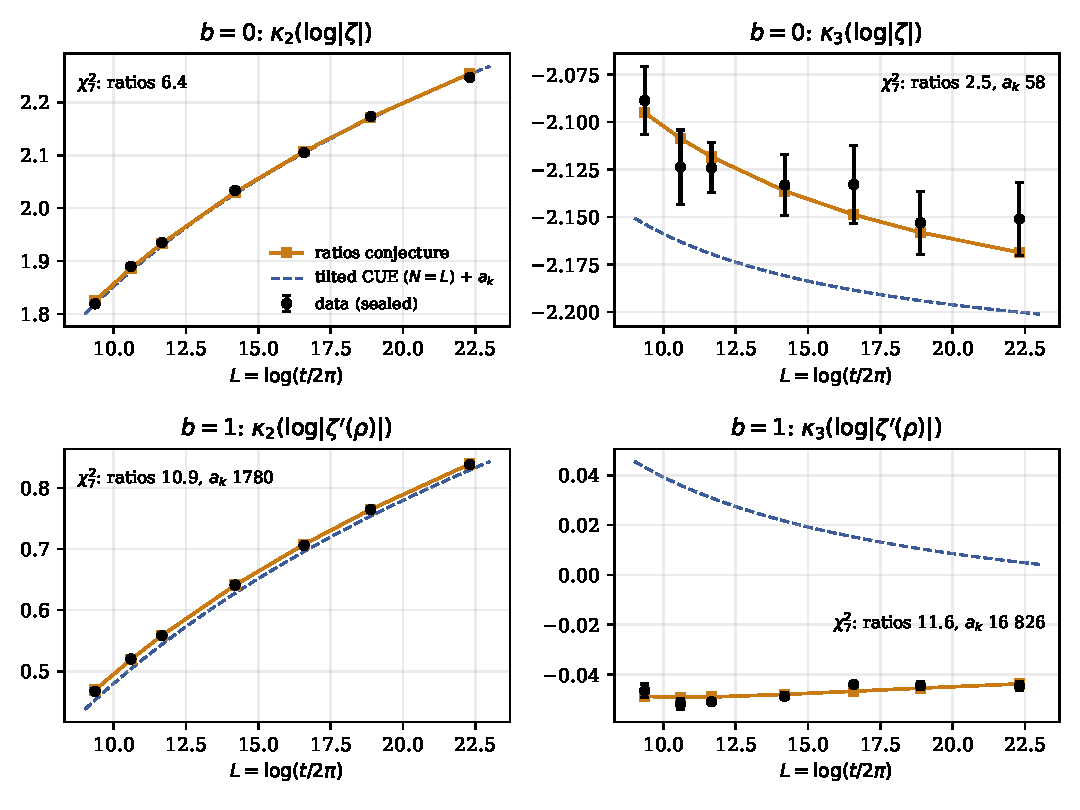
\includegraphics[width=\textwidth]{figures/ladder_ratios.pdf}
\caption{\label{fig:ladder}The first two rungs of the ladder at finite
height. Points: sealed data from Tests 200-A and 200-C (seven windows).
Squares: ratios-conjecture predictions, committed before comparison, no
free parameters. Dashed: tilted CUE at $N=L$ plus the Keating--Snaith
arithmetic cumulants, the model that is correct as $L\to\infty$.}
\end{figure}

\begin{table}[h]
\centering
\footnotesize
\setlength{\tabcolsep}{4pt}
\begin{tabular}{lcccc}
\toprule
& \multicolumn{2}{c}{$b=0$: $\log|\zeta(\frac12+it)|$} & \multicolumn{2}{c}{$b=1$: $\log|\zeta'(\rho)|$}\\
$L$ & $\kappa_2$ & $\kappa_3$ & $\kappa_2$ & $\kappa_3$\\
\midrule
$9.35$ & 1.8191(45) / 1.8249 & $-$2.089(18) / $-$2.095 & 0.4672(22) / 0.4691 & $-$0.0465(27) / $-$0.0488\\
$10.59$ & 1.8899(44) / 1.8858 & $-$2.124(20) / $-$2.109 & 0.5200(14) / 0.5190 & $-$0.0519(21) / $-$0.0492\\
$11.66$ & 1.9348(39) / 1.9330 & $-$2.124(13) / $-$2.118 & 0.5586(11) / 0.5584 & $-$0.0509(10) / $-$0.0490\\
$14.19$ & 2.0333(40) / 2.0300 & $-$2.133(16) / $-$2.136 & 0.64107(55) / 0.64099 & $-$0.0487(13) / $-$0.0480\\
$16.58$ & 2.1051(42) / 2.1068 & $-$2.133(20) / $-$2.149 & 0.70628(54) / 0.70783 & $-$0.0440(12) / $-$0.0467\\
$18.88$ & 2.1729(40) / 2.1714 & $-$2.153(17) / $-$2.158 & 0.76478(61) / 0.76496 & $-$0.0445(15) / $-$0.0454\\
$22.31$ & 2.2471(43) / 2.2542 & $-$2.151(19) / $-$2.169 & 0.83829(82) / 0.83925 & $-$0.0446(19) / $-$0.0437\\
\midrule
$\chi^2_7$ & $6.4$ & $2.5$ & $10.9$ & $11.6$\\
\bottomrule
\end{tabular}
\caption{\label{tab:ratios}Observed / ratios-conjecture values of the
second and third cumulants of $\log|\zeta(\frac12+it)|$ at random $t$
(rung $b=0$) and of $\log|\zeta'(\rho)|$ over zeros (rung $b=1$). The
predictions were committed before comparison and have no free parameters
(Appendix~\ref{app:ratios}); for $b=1$, $\kappa_3$ the committed values are
shown, and the post-audit correction gives $\chi^2=10.9$. As
$L\to\infty$, $\kappa_3$ at $b=0$ tends to $-\pi^2/4+c_P=-2.2337$ (the
prediction is $-2.2072$ at $L=60$ and $-2.2186$ at $L=120$).}
\end{table}

%======================================================================
\section{Reading and open problems}\label{sec:open}
%======================================================================

The ``halving at each conditioned zero'' seen at $L\approx11$ is a
finite-height effect: as the height grows the ladder flattens, the ratios
rising from $0.53/0.57$ to $0.65/0.80$ (Table~\ref{tab:shifts}), the
differences between rungs close like $L^{-\nu}$ with $\nu\approx0.45$--$0.75$,
and the three rungs approach a common value, as in the asymptotic picture of
Keating--Snaith and Hughes--Keating--O'Connell. For $b=0$ and $b=1$ the
finite-height values are now derived from the ratios conjecture: the plateau of the $b=0$ shift at
$\approx0.28$ is an artefact of subtracting the CUE at $N=L$, whose own
$1/N$ term ($+\frac34/N$ for $\kappa_3$) differs from that of $\zeta$. For
$b=2$ the geometric decay of 200-B and the relaxation law of 200-C remain
extrapolations: each passed a blind test on unseen data, but neither is
derived. Open problems:
\begin{enumerate}
\item \emph{Finite-$\eps$ corrections.} Prove that the corrections in
Theorem~\ref{thm:main} are $O(\eps^2)$ and compute the leading
coefficient.
\item \emph{Close pairs of zeta.} Extend the ratios-conjecture computation
of Appendix~\ref{app:ratios} to $b=2$, which needs the two-point density
of zeros and hence four- and five-point averages, and derive the rung
dependence of the $\kappa_3$ shift and its relaxation; decide whether the
phase lock of Test 201 is the mechanism; prove
Conjecture~\ref{conj:zeta}(ii) for small $k$ under a hypothesis, in the
manner of \cite{BGM15} for $\zeta'(\rho)$.
\item \emph{Rigour.} Make the $b=0$ and $b=1$ computations rigorous under
explicit hypotheses, as \cite{FG24} did for the limit at $b=0$.
\item \emph{Phase lock of close pairs.} Derive the factor $4$ of Test 201
and its $\eps$-dependence beyond the local-GUE heuristic.
\item \emph{All gaps.} Theorem~\ref{thm:main} is the small-gap end of the
open problem of \cite{companion1}: the mean of $M_n^2$ conditioned on a
gap of any size.
\end{enumerate}

\appendix
\section{Cumulants of $\log|\zeta|$ at finite height from the ratios
conjecture}\label{app:ratios}

Let $L=\log(t/2\pi)$, $X(\alpha)=\frac{\zeta'}\zeta(\frac12+\alpha+it)$ and
$\bar X(\beta)=\frac{\zeta'}\zeta(\frac12+\beta-it)$ for real shifts, and let
$\E$ denote the average over $t$ in a window at height $L$. Since
$\log\zeta(s)=-\int_0^\infty\frac{\zeta'}\zeta(s+a)\,da$ and averages of
products of unconjugated factors vanish,
\begin{equation}\label{eq:k23}
\kappa_2=\tfrac12\iint_{\mathbb R_+^2}\E[X(a)\bar X(b)]\,da\,db,\qquad
\kappa_3=-\tfrac34\iiint_{\mathbb R_+^3}\E[X(a)X(b)\bar X(c)]\,da\,db\,dc
\end{equation}
for the cumulants of $\log|\zeta(\frac12+it)|$ (the mean is $0$). We
evaluate the averages with the ratios conjecture \cite{CFZ08}: the recipe
replaces $\E\prod\zeta(s+\alpha_k)\prod\zeta(1-s+\beta_l)/(\cdots)$ by a sum
over swaps $\alpha_S\leftrightarrow-\beta_T$ ($|S|=|T|$), each weighted by
$(t/2\pi)^{-\sum_S\alpha-\sum_T\beta}$ and by a product of $\zeta(1+\cdot)$
factors and an absolutely convergent Euler product $A$; the averages of
$\zeta'/\zeta$ follow by differentiating and setting the denominator shifts
equal to the numerator shifts. Put $F(x)=e^{-Lx}\zeta(1+x)\zeta(1-x)A(x)$
with
\[
A(x)=\prod_p\frac{(1-p^{-1-x})(1-2p^{-1}+p^{-1-x})}{(1-p^{-1})^2}.
\]

\emph{Two points} \cite{CS07}. $\E[X(\alpha)\bar X(\beta)]=G(\alpha+\beta)$
with $G(x)=\sum_p\frac{\log^2p}{p^{1+x}-1}+F(x)$, so
$\kappa_2=\frac12\int_0^\infty x\,G(x)\,dx$.

\emph{Three points.} With $x_i=\alpha_i+\beta$,
\begin{equation}\label{eq:three}
\E[X(\alpha_1)X(\alpha_2)\bar X(\beta)]=D+F(x_1)\,K(\alpha_2-\alpha_1,x_1)
+F(x_2)\,K(\alpha_1-\alpha_2,x_2),
\end{equation}
\begin{gather*}
D=-\sum_p\log^3p\,\frac{y_1y_2}{(1-y_1)(1-y_2)},\qquad y_i=p^{-1-x_i},\\
K(u,x)=-\sum_p\log p\,\frac{q}{1-q}\,
\frac{(1-p^{-1})(1-p^{-x})}{1-2p^{-1}+p^{-1-x}},\qquad q=p^{-1-u}.
\end{gather*}
The identity term $D$ is the average under independent uniform phases
$p^{-it}$. The swap term $\alpha_1\leftrightarrow-\beta$ vanishes to second
order at the diagonal through the factors $1/\zeta(1-\beta+\delta)$ and
$1/\zeta(1-\alpha_1+\gamma_1)$, which absorb $\partial_\beta$ and
$\partial_{\alpha_1}$; $\partial_{\alpha_2}$ acts on the rest. For each
prime the local average of the swapped Euler factor has the closed form
$1+(1-p^{-\alpha_1-\delta})\bigl[\frac{(1-p^{-1+\alpha_1-\gamma_1})
(1-p^{-1+\alpha_1-\gamma_2})}{(1-p^{-1+\alpha_1+\beta})(1-p^{-1+\alpha_1-\alpha_2})}-1\bigr]$,
and $\frac{\zeta'}\zeta(1+\alpha_2-\alpha_1)-\frac{\zeta'}\zeta(1+\alpha_2+\beta)
+\partial_{\alpha_2}\log A_{\rm swap}$ collapses to $K$ (we checked both
steps numerically, prime by prime, to $10^{-10}$). For $u<0$ the kernel is
continued as $K=\frac{\zeta'}\zeta(1+u)+P(1+u+x)+Q_2-C$, with
$P(s)=\sum_p\log p\,p^{-s}$ and two sums $Q_2,C$ that converge for
$u>-1$.

\emph{The integral.} Integrating $D$ term by term gives
$\frac34\sum_p\sum_{m_1,m_2\ge1}\frac{p^{-m_1-m_2}}{m_1m_2(m_1+m_2)}=c_P$
exactly. The swap terms are not separately absolutely integrable near the
origin: splitting them and taking a principal value at $\alpha_1=\alpha_2$
loses exactly $-\pi^2/4$. The correct form uses the combined kernel
$\Phi(x_1,x_2)=F(x_1)K(x_2-x_1,x_1)+F(x_2)K(x_1-x_2,x_2)$, finite on the
diagonal; with $x_1=a+c$, $x_2=b+c$ the $c$-integral gives
$\min(x_1,x_2)$ and
\[
\kappa_3=c_P-\tfrac32\int_0^\infty x_1\,dx_1\int_0^\infty
\Phi(x_1,x_1+w)\,dw.
\]
With $\zeta(1+x)\mapsto(1-e^{-x})^{-1}$, $A\mapsto1$ and $L\mapsto N$
the same formula reproduces the exact CUE values
$\kappa_3(N)=\frac34\sum_{j\le N}\psi''(j)$ for $N=1,2,5,10$ to five
decimals. Numerical details (prime cut-off, quadrature, cuts) and their
sensitivities, all below $10^{-3}$, are in Section~\ref{S-sec:numsupp}.

\emph{Averages over zeros.} From the Hadamard product,
$\sum_\gamma\frac{c}{c^2+(t-\gamma)^2}=\mathrm{Re}\frac{\zeta'}\zeta(\frac12+c+it)
+\frac L2+O(1/t)$, so as $c\to0^+$ the zeros have density
$\frac1{2\pi}[L+2\,\mathrm{Re}X(0)]$ and
$\E_\rho[M]=\E[M]+\frac1L(\E[MX(0)]+\E[M\bar X(0)])$ (for the CUE this is
exact, with $N$ for $L$). With
$\log\zeta'(\rho)=-\int_0^\infty[\frac{\zeta'}\zeta(\rho+a)-\1_{a<1}/a]\,da$,
the variance of $\log|\zeta'(\rho)|$ is
$\frac12[\mathrm{Cov}(Y,\bar Y)+\mathrm{Cov}(Y,Y)]$, where
$\E_\rho[X(a)]=G(a)/L$,
$\E_\rho[X(a)\bar X(b)]=G(a+b)+[T(a,0;b)+T(b,0;a)]/L$ and
$\E_\rho[X(a)X(b)]=T(a,b;0)/L$, with $T(\alpha_1,\alpha_2;\beta)$ the
three-point average \eqref{eq:three}. The integrand is symmetric, and near
$a=0$ terms of order $1/a$ cancel. In the CUE analogue this reproduces
$\sum_{j<N}[\psi'(j+2)-\frac12\psi'(j+1)]$ to six decimals. As an
independent check, the averages $\E_\rho[X(a)\bar X(b)]$ entering the
integrand were computed directly from $8\cdot10^5$ zeros at $L=14.19$ (where
$\mathrm{Re}X_\rho$ is an exact sum over zeros): for $a,b$ between $0.1/L$
and $6/L$ all fifteen cells agree with the formula within their
statistical errors, whereas the CUE at $N=L$ is off by about $25\%$.

\emph{Four points: the third cumulant over zeros.} Here
$\E_\rho[X(a)X(b)\bar X(c)]=T(a,b;c)+[Q(a,b,0;c)+Q_2(a,b;c,0)]/L$ and
$\E_\rho[X(a)X(b)X(c)]=Q(a,b,c;0)/L$, with the four-point averages
\begin{align*}
Q(\alpha_1,\alpha_2,\alpha_3;\beta)&=D_4+\sum_iF(x_i)\bigl[f^{(i)}_{jk}
+K(\alpha_j-\alpha_i,x_i)K(\alpha_k-\alpha_i,x_i)\bigr],\\
Q_2(\alpha_1,\alpha_2;\beta_1,\beta_2)&=H_{11}H_{22}+H_{12}H_{21}+\sum_pc_{4,p}+S_{\rm dbl}\\
&\quad+\sum_{i,j}F(x_{ij})\bigl[f_{i'j'}+K(\alpha_{i'}-\alpha_i,x_{ij})K(\beta_{j'}-\beta_j,x_{ij})\bigr],
\end{align*}
where $x_{ij}=\alpha_i+\beta_j$, $H$ is the identity part of $G$, $D_4$ and
$c_{4,p}$ are the connected four-point terms of the independent-phase model,
$f^{(i)}_{jk}=\sum_p\log^2p\,\omega_p(x_i)\frac{q_jq_k}{(1-q_j)(1-q_k)}$ with
$q_j=p^{-1-\alpha_j+\alpha_i}$ and
$\omega_p(x)=\frac{(1-p^{-x})(1-p^{-1})p^{-x}(1-p^{-1+x})}{(1-2p^{-1}+p^{-1-x})^2}$,
$f_{i'j'}=\sum_p\partial_{\alpha_{i'}}\partial_{\beta_{j'}}\log E_p$ is a
closed form in the local factors (in the CUE it reduces to $H(x_{i'j'})$), and
the double swap is
$S_{\rm dbl}=e^{-L(\alpha_1+\alpha_2+\beta_1+\beta_2)}\prod_{k,l}\zeta(1\pm x_{lk})
/[\zeta(1\pm(\beta_1-\beta_2))\zeta(1\pm(\alpha_1-\alpha_2))]\,A_{\rm dbl}$.
The Euler product for $A_{\rm dbl}$ converges only when all $x_{lk}<\frac12$;
outside that region we interpolate between its exact limits
$A(x_{21})$ as $x_{12}\to0$ and $A(x_{11})$ as $x_{22}\to0$ (checked
numerically), which moves $\kappa_3$ by at most $3\cdot10^{-4}$. Numerically we
write $\kappa_3=\kappa_3^{\rm CUE}(L)+\iiint(I_\zeta-I_{\rm CUE})$: the CUE
part is the exact Palm value, and only the difference of the integrands is
integrated numerically. This is a derivation under the ratios conjecture,
with limits and integrals interchanged freely; it is not a theorem.

\section*{Data availability statement}

The data that support the findings of this study are openly available at
\href{https://doi.org/10.5281/zenodo.22942475}{doi:10.5281/zenodo.22942475},
the archive of the repository
\url{https://github.com/azizran/riemann-zero-statistics} (directory
\texttt{qm\_riemann/}). It contains all code, data products,
pre-registration files (with sha256 stamps and dates) and the research log,
including the failed predictions; the LMFDB zero files are not
redistributed, but their sha256 stamps are given. The ratios-conjecture
predictions were committed before comparison to the author's private
working repository (commits \texttt{182190f}, \texttt{bf214f0},
\texttt{a056eb0}, \texttt{e5f2580}; post-audit correction
\texttt{62b36dd}). A file-by-file guide is in Section~\ref{S-sec:repro}.

\section*{Acknowledgements}

The question that started this note was asked by a reader; we thank them
for it. Computations, derivation audits, literature search and drafting
were done with the help of an AI assistant (Claude Opus 5.5, Anthropic,
used through Claude Code); derivations, pre-registrations and literature
searches were audited by independent instances of a Claude Sonnet model
before predictions were frozen. All results were checked by the author,
who takes full responsibility for the content; errors are the author's.

\begin{thebibliography}{99}

\bibitem{companion1} U.~Sezen, \emph{The joint law of zero gaps and local
maxima of Hardy's $Z$-function}, preprint (2026); archived at Zenodo,
\href{https://doi.org/10.5281/zenodo.22942475}{doi:10.5281/zenodo.22942475}.

\bibitem{companion2} U.~Sezen, \emph{The prime-wave anatomy of the
gap--amplitude law for Riemann zeros}, preprint (2026); archived at Zenodo,
\href{https://doi.org/10.5281/zenodo.22942475}{doi:10.5281/zenodo.22942475}.

\bibitem{Bar00} E.~W.~Barnes, \emph{The theory of the $G$-function},
Quart.\ J.\ Pure Appl.\ Math.\ \textbf{31} (1900), 264--314.

\bibitem{BAB13} G.~Ben Arous, P.~Bourgade, \emph{Extreme gaps between
eigenvalues of random matrices}, Ann.\ Probab.\ \textbf{41} (2013), no.~4,
2648--2681, doi:\nolinkurl{10.1214/11-AOP710}.

\bibitem{BW26} T.~Bothner, F.~Wei, \emph{Joint moments of characteristic
polynomials in the circular Jacobi ensemble and Painlev\'e equations},
arXiv:2608.24423 (2026).

\bibitem{Bou22} P.~Bourgade, \emph{Extreme gaps between eigenvalues of
Wigner matrices}, J.\ Eur.\ Math.\ Soc.\ \textbf{24} (2022), no.~8,
2823--2873, doi:\nolinkurl{10.4171/JEMS/1141}.

\bibitem{BHNY08} P.~Bourgade, C.~P.~Hughes, A.~Nikeghbali, M.~Yor,
\emph{The characteristic polynomial of a random unitary matrix: a
probabilistic approach}, Duke Math.\ J.\ \textbf{145} (2008), no.~1,
45--69, doi:\nolinkurl{10.1215/00127094-2008-046}; arXiv:0706.0333 (statement numbers
cited here are those of the arXiv version).

\bibitem{BNR09} P.~Bourgade, A.~Nikeghbali, A.~Rouault, \emph{Circular
Jacobi ensembles and deformed Verblunsky coefficients}, Int.\ Math.\ Res.\
Not.\ IMRN \textbf{2009}, no.~23, 4357--4394, doi:\nolinkurl{10.1093/imrn/rnp092};
arXiv:0804.4512 (statement numbers cited here are those of the arXiv
version).

\bibitem{BGM15} H.~M.~Bui, S.~M.~Gonek, M.~B.~Milinovich, \emph{A hybrid
Euler--Hadamard product and moments of $\zeta'(\rho)$}, Forum Math.\
\textbf{27} (2015), 1799--1828, arXiv:1302.5032.

\bibitem{CFZ08} J.~B.~Conrey, D.~W.~Farmer, M.~R.~Zirnbauer,
\emph{Autocorrelation of ratios of $L$-functions}, Commun. Number Theory
Phys. \textbf{2} (2008), 593--636.

\bibitem{CS08} J.~B.~Conrey, N.~C.~Snaith, \emph{Correlations of eigenvalues
and Riemann zeros}, arXiv:0803.2795 (2008).

\bibitem{CS07} J.~B.~Conrey, N.~C.~Snaith, \emph{Applications of the
$L$-functions ratios conjectures}, Proc. London Math. Soc. (3) \textbf{94}
(2007), 594--646.

\bibitem{CG85} J.~B.~Conrey, A.~Ghosh, \emph{A mean value theorem for the
Riemann zeta-function at its relative extrema on the critical line},
J.\ London Math.\ Soc.\ (2) \textbf{32} (1985), 193--202.

\bibitem{FTW19} R.~Feng, G.~Tian, D.~Wei, \emph{Small gaps of GOE},
Geom.\ Funct.\ Anal.\ \textbf{29} (2019), no.~6, 1794--1827,
doi:\nolinkurl{10.1007/s00039-019-00520-5}.

\bibitem{FW21} R.~Feng, D.~Wei, \emph{Small gaps of circular
$\beta$-ensemble}, Ann.\ Probab.\ \textbf{49} (2021), no.~2, 997--1032,
doi:\nolinkurl{10.1214/20-AOP1468}.

\bibitem{FG24} A.~Fazzari, M.~Gerspach, \emph{The third moment of the
logarithm of zeta and a twisted pair correlation conjecture},
arXiv:2412.20099 (2024).

\bibitem{For10} P.~J.~Forrester, \emph{Log-Gases and Random Matrices},
London Math.\ Soc.\ Monographs Ser.\ \textbf{34}, Princeton University
Press, Princeton, NJ, 2010.

\bibitem{GHK07} S.~M.~Gonek, C.~P.~Hughes, J.~P.~Keating, \emph{A hybrid
Euler--Hadamard product for the Riemann zeta function}, Duke Math.\ J.\
\textbf{136} (2007), 507--549.

\bibitem{Gonek93} S.~M.~Gonek, \emph{An explicit formula of Landau and its
applications to the theory of the zeta-function}, in: M.~Knopp et al.\
(eds.), A Tribute to Emil Grosswald: Number Theory and Related Analysis,
Contemp.\ Math.\ \textbf{143}, Amer.\ Math.\ Soc., Providence, RI, 1993,
395--413.

\bibitem{HKO00} C.~P.~Hughes, J.~P.~Keating, N.~O'Connell, \emph{Random
matrix theory and the derivative of the Riemann zeta function},
Proc.\ R.\ Soc.\ Lond.\ A \textbf{456} (2000), 2611--2627.

\bibitem{HLPC24} C.~Hughes, S.~Lugmayer, A.~Pearce-Crump, \emph{The second
moment of the Riemann zeta function at its local extrema}, J.\ London
Math.\ Soc.\ (2) \textbf{112} (2025), e70250, arXiv:2411.05573.

\bibitem{KS00} J.~P.~Keating, N.~C.~Snaith, \emph{Random matrix theory and
$\zeta(1/2+it)$}, Comm.\ Math.\ Phys.\ \textbf{214} (2000), 57--89.

\bibitem{Landau12} E.~Landau, \emph{\"Uber die Nullstellen der
Zetafunktion}, Math.\ Ann.\ \textbf{71} (1912), 548--564,
doi:\nolinkurl{10.1007/BF01456808}.

\bibitem{LMFDB} The LMFDB Collaboration, \emph{The $L$-functions and modular
forms database}, \url{https://www.lmfdb.org}, 2026, [Online; accessed
27 September 2026].

\bibitem{Mez07} F.~Mezzadri, \emph{How to generate random matrices from the
classical compact groups}, Notices Amer.\ Math.\ Soc.\ \textbf{54} (2007),
592--604, arXiv:math-ph/0609050.

\bibitem{Odl87} A.~M.~Odlyzko, \emph{On the distribution of spacings
between zeros of the zeta function}, Math.\ Comp.\ \textbf{48} (1987),
273--308.

\bibitem{OdlyzkoTables} A.~M.~Odlyzko, \emph{Tables of zeros of the Riemann
zeta function}, \url{https://www-users.cse.umn.edu/~odlyzko/zeta_tables/}.

\bibitem{Pla15} D.~J.~Platt, \emph{Computing $\pi(x)$ analytically},
Math.\ Comp.\ \textbf{84} (2015), no.~293, 1521--1535,
doi:\nolinkurl{10.1090/S0025-5718-2014-02884-6}.

\bibitem{Win12} B.~Winn, \emph{Derivative moments for characteristic
polynomials from the CUE}, Comm.\ Math.\ Phys.\ \textbf{315} (2012),
no.~2, 531--562, doi:\nolinkurl{10.1007/s00220-012-1512-1}; arXiv:1109.0227.

\end{thebibliography}

\end{document}
